%ctrl+alt+m:open Math Preview
\documentclass[a4paper,11pt,uplatex]{jsarticle}%titlepage
%:/usr/local/texlive/texmf-local/tex/latex/report/report.sty
\usepackage{myreport}
\title{拡散モデル(Diffusion Model)を理解するために}
\author{20B01392 松本侑真}
\date{\today}
\begin{document}
\maketitle
\begin{abstract}
  近年、機械学習を応用した生成系AIがブームである。
  生成系AIを使うことで、プロンプトに入力したテキストデータから画像データなどを出力することができる。
  拡散モデルを用いた有名な生成系AIのStable Diffusionでは、無料でプロンプトに入力した文字(例:かわいい犬)から、かわいい犬の画像を出力することができる。
  このような生成系AIで用いられる拡散モデルについて理解するための基礎を説明する。
\end{abstract}
\tableofcontents
\newpage

\section{生成モデルでは何を行っているのか}
生成モデル(拡散モデル)は、事前に与えられた教師データを元にモデルを学習することで、
未知の入力に対して最適化された出力をアウトプットすることができる。
例えば、いろいろな人間の顔データを学習させた生成モデルを用いると、
「40歳のおじさん」や「20代のアイドル」といった入力を元にして、学習されたモデルで生成した顔画像を出力する。

生成モデルの学習というのは、「モデルの入力から欲しいデータを生み出す確率分布」をいかにして見つけるかということである。
すなわち、任意のデータ$\vv{x}$は、とある1つの確率分布$p(\vv{x})$に従って生み出されるという仮定のもと、自分のモデルをその$p(\vv{x})$に限りなく近づけることが生成モデルにおける学習である。
すなわち、あらゆるデータが従う確率分布$p(\vv{x})$そのものを手に入れることができれば、$p(\vv{x})$の値を出力するような$\vv{x}$を見つけることが可能であるだろう。
これによって、$p(\vv{x})=\text{「20代のアイドル」}$を満たす画像$\vv{x}$を出力することができる。

\subsubsection*{学習を行う前に得られているもの}
モデルの学習を行うためには、そのための学習データが必要である。$n$個の学習データ$\vv{x}_1,\,\vv{x}_2,\,\cdots,\,\vv{x}_n$が手元にあるとする。
このとき、
\begin{equation}
  p_0(\vv{x}) = \frac{1}{n}\sum_{i=1}^{n}\delta(\vv{x}-\vv{x}_i)
\end{equation}
を経験分布と呼ぶ。この経験分布は、$n$が十分に大きいとき、あらゆるデータを生み出す確率分布$p(x)$に非常に近いであろう:
\begin{equation}
  p_0(\vv{x}) \approx p(\vv{x})\;。
\end{equation}
なお、データを連続変数として扱う場合は$\delta(\vv{x}-\vv{x}_i)$をデルタ関数、離散変数として扱う場合はクロネッカーのデルタとして扱う。

\subsubsection*{学習のために必要なもの}
生成モデルにおいて学習させるための確率分布は自ら用意する必要がある。すなわち、パラメータ$\theta$を用いて、
\begin{equation}
  p(\vv{x})\approx q_{\theta}(\vv{x})
\end{equation}
となるようなモデル$q_{\theta}(\vv{x})$を見つけたい。モデル$q_{\theta}(\vv{x})$の関数形は計算しやすい形を用いて、
パラメータ$\theta$を最適化することで$p(\vv{x})$に近づけるというアプローチを取る。

\section{ボルツマンマシン}
ボルツマンマシンとは、モデル$q_{\theta}(\vv{x})$が
\begin{equation}
  q_{\theta}(\vv{x}) = \frac{1}{Z_{\theta}}\exp(-E_{\theta}(\vv{x}))\;。
\end{equation}
と表されるものである。このような関数形をGibbs-Boltzmann分布(指数関数分布族)と呼ぶ。
ここで、規格化定数$Z_{\theta}$は
\begin{equation}
  Z_{\theta} = \sum_{\vv{x}}\exp(-E_{\theta}(\vv{x}))
\end{equation}
である。このように定義された$q_{\theta}(\vv{x})$を$p(\vv{x})$に近づけることが目標である。
しかし、$p(\vv{x})$の形は誰も知らない。今手元にあるのは経験分布$p_0(\vv{x})$だけである。
そのため、学習データの数$n$が十分に多いとして、$q_{\theta}(\vv{x})$を経験分布$p_0(\vv{x})$に近づけることを行う。

\subsection{Kullback-Leibler情報量}
学習を行うためには、2つの確率分布$p(\vv{x}),\,q(\vv{x})$の近さを定義する必要がある。
この「近さ」は、データ$\vv{x}$を入力した際の2つの確率分布間の「距離$D(p\parallel q)$」を測ることで定義することができるだろう。
このような関数$D(p\parallel q)$はどのように設定しても良いのだが、
今回は、Kullback-Leibler divergence(KL情報量)$D_{\text{KL}}(p\parallel q)$を導入する:
\begin{equation}
  D_{\text{KL}}(p(\vv{x})\parallel q(\vv{x})) = \sum_{\vv{x}}p(\vv{x})\ln\frac{p(\vv{x})}{q(\vv{x})}\;。
\end{equation}
KL情報量には
\begin{enumerate}
  \item $D(p\parallel q)\geq 0$(等号成立は$p=q$のとき)
  \item $D(p\parallel q) \neq D(q\parallel p)$(非対称性)
\end{enumerate}
といった性質がある。特に、KL情報量は$0$以上であるといった性質を良く用いる。この性質を2つの方法で証明してみる。
\subsubsection*{Gibbsの不等式を用いる方法}
Gibbsの不等式とは、$x>0$において
\begin{equation}
  x-1\geq \ln{x}\Longleftrightarrow \ln{\frac{1}{x}}\geq 1-x
\end{equation}
が成立する不等式である。
\begin{figure}[H]
  \centering
  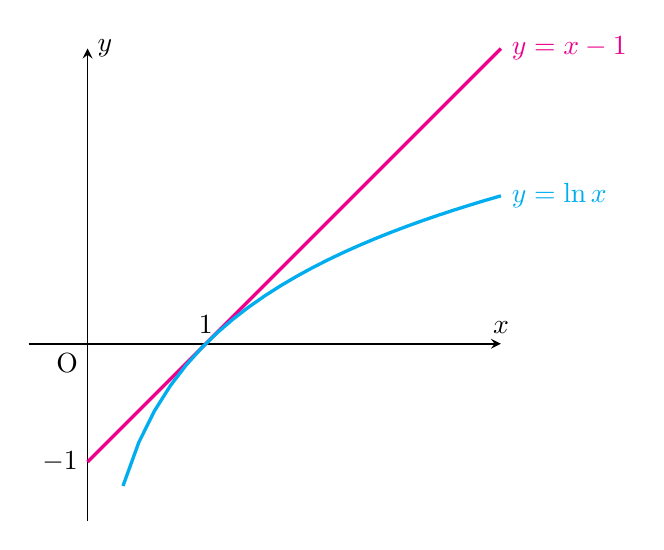
\begin{tikzpicture}[scale=1.5]
    \draw[->,>=stealth,semithick](-0.5,0)--(3.5,0)node[above]{$x$};%x軸
    \draw[->,>=stealth,semithick](0,-1.5)--(0,2.5)node[right]{$y$};%y軸
    \draw(0,0)node[below left]{O};%原点
    \draw(1,0)node[above]{$1$};
    \draw(0,-1)node[left]{$-1$};
    \draw[magenta,very thick,domain=0:3.5]plot(\x,\x-1)node[right]{$y=x-1$};
    \draw[cyan,very thick,domain=0.3:3.5]plot(\x,{ln(\x)})node[right]{$y=\ln{x}$};
  \end{tikzpicture}
  \caption{Gibbsの不等式の直感的な理解}
\end{figure}
Gibbsの不等式を用いると、
\begin{equation}
  D_{\text{KL}}(p\parallel q) = \sum_{\vv{x}}p(\vv{x})\ln\frac{p(\vv{x})}{q(\vv{x})}
  \geq \sum_{\vv{x}}p(\vv{x})\qty(1-\frac{q(\vv{x})}{p(\vv{x})})
  = \sum_{\vv{x}}p(\vv{x})-\sum_{\vv{x}}q(\vv{x}) =0
\end{equation}
と示される。
\newpage
\subsubsection*{Jensenの不等式を用いる方法}
Jensenの不等式とは、上に凸な関数$f(x)$に対して、
\begin{equation}
  f\qty(\frac{a+b}{2})\geq \frac{f(a)+f(b)}{2}
\end{equation}
が成立する不等式である。
\begin{figure}[H]
  \centering
  \begin{tikzpicture}[scale=1.5]
    \coordinate(A)at(-2,0);
    \coordinate(B)at(1,0);
    \draw[->,>=stealth,semithick](-3.5,0)--(3.5,0)node[above]{$x$};%x軸
    \draw[magenta,very thick,domain=-3:3]plot(\x,{-0.3*(\x-3)*(\x+3)});
    \coordinate(YA)at(-2,1.5);
    \coordinate(YB)at(1,2.4);
    \draw[dashed](A)node[below]{$a$}--(YA);
    \draw[dashed](B)node[below]{$b$}--(YB);
    \draw[dashed](YA)--(YB);
    \fill(YA)circle(0.05);
    \fill(YB)circle(0.05);
    \coordinate(XAB)at($(A)!1/2!(B)$);
    \coordinate(YAB)at($(XAB)+(0,0.3*7/2*5/2)$);
    \draw[dashed](XAB)node[below]{$\frac{a+b}{2}$}--(YAB);
    \fill(YAB)circle(0.05);
  \end{tikzpicture}
  \caption{Jensenの不等式の直感的な理解}
\end{figure}
Jensenの不等式を用いると、
\begin{equation}
  D_{\text{KL}}(p\parallel q) = -\sum_{\vv{x}}p(\vv{x})\ln\frac{q(\vv{x})}{p(\vv{x})}
  \geq -\ln\qty(\sum_{\vv{x}}p(\vv{x})\frac{q(\vv{x})}{p(\vv{x})}) = 0
\end{equation}
と示される。

\subsection{例:ガウス分布のKL情報量と学習}
モデル$q_{\theta}(\vv{x})$をガウス分布とおいて最適化を行う。人間が計算できるのはせいぜいガウス分布程度であるため、
これ以上難しいモデルは考えない。まずは$\vv{x}$が1次元のスカラーである場合を考える:
\begin{equation}
  q_{\theta}(x)\propto \exp\qty(-\frac{1}{2\sigma^2}(x-\mu)^2)\;。
\end{equation}
規格化定数は
\begin{equation}
  Z_{\theta}=\int_{-\infty}^{\infty}dx\,\exp\qty(-\frac{1}{2\sigma^2}(x-\mu)^2) = \sqrt{2\pi\sigma^2}
\end{equation}
となる。したがって、
\begin{equation}
  q_{\theta}(x)=\frac{1}{\sqrt{2\pi\sigma^2}}\exp\qty(-\frac{1}{2\sigma^2}(x-\mu)^2)
\end{equation}
となる。このモデルの未知数は$\mu$と$\sigma^2$であるため、最適化すべきパラメータは$\theta=\{\mu,\,\sigma^2\}$となる。
次に、KL情報量を考える。$q_{\theta}(x)$を$p(x)$に近づけることができれば良いのだが、あいにく$p(x)$の具体形はわからない。
そのため、経験分布$p_0(x)=\sum_{i=1}^n\delta(x-x_i)$にモデルを近づけることを考える。KL情報量を計算すると、
\begin{align}
  D_{\text{KL}}(p_0\parallel q_{\theta}) = \int dx\,p_0(x)\qty(\ln{p_0(x)}-\ln{q_{\theta}(x)})
   & \underbrace{=}_{\theta\text{のみ}} -\int dx\,p_0(x)\qty(\frac{1}{2\sigma^2}(x-\mu)^2+\frac{1}{2}\ln{\sigma^2}) \notag \\
   & \;\,=\frac{1}{2\sigma^2}\frac{1}{n}\sum_{i=1}^n(x_i-\mu)^2+\frac{1}{2}\ln{\sigma^2}
\end{align}
となる。KL情報量を最小化(学習)すれば、経験分布に近いモデルが得られるため、$\mu$と$\sigma^2$で偏微分を行う。
\begin{align}
  \pdv{D_{\text{KL}}}{\mu}      & = -\frac{1}{\sigma^2}\frac{1}{n}\sum_{i=1}^{n}(x_i-\mu) = 0
                                &                                                                                      & \Longleftrightarrow \mu = \frac{1}{n}\sum_{i=1}^nx_i\;\text{(データの平均)}              \\
  \pdv{D_{\text{KL}}}{\sigma^2} & = -\frac{1}{2(\sigma^2)^2}\frac{1}{n}\sum_{i=1}^n(x_i-\mu)^2 + \frac{1}{2\sigma^2}=0
                                &                                                                                      & \Longleftrightarrow \sigma^2 = \frac{1}{n}\sum_{i=1}^n(x_i-\mu)^2\;\text{(データの分散)}
\end{align}
この結果からわかることは、ガウス分布のモデルの平均$\mu$はデータの平均値に、モデルの分散$\sigma^2$はデータの分散にすれば、
$p(x)$に近いモデル$q_{\theta}(x)$を生成できるということである。

\subsection{最尤法(=KL最小化)}
最尤法とは、KL情報量の最小化と同値なものであるが、良く使われるため紹介する。モデルの学習は、
\begin{equation}
  \min_{\theta}\qty{D_{\text{KL}}(p_0(\vv{x})\parallel q_{\theta}(\vv{x}))}
  = \max_{\theta}\qty{\sum_{\vv{x}}p(\vv{x})\ln{q_{\theta}(\vv{x})}}
  = \max_{\theta}\qty{\frac{1}{n}\sum_{i=1}^n\ln{q_{\theta}(\vv{x}_i)}}
\end{equation}
と変形することができる。$\ln{q_{\theta}(\vv{x}_i)}$を対数尤度関数と呼び、モデルの良さの指標として使われる。
対数尤度を最大化することは、KL情報量の最小化と同値なものである。
\subsection{高次元化}
先ほどはガウス分布のモデルの1次元バージョンの最適化を行った。一般の場合にどのように拡張されるかを見る。
すなわち、
\begin{equation}
  q_{\theta}(\vv{x}) \propto \exp\qty(-\frac{1}{2}(\vv{x}-\vv{\mu})^{\top}\Sigma^{-1}(\vv{x}-\vv{\mu}))
\end{equation}
とする。規格化定数は
\begin{equation}
  Z_{\theta} = \int d\vv{x}\,\exp\qty(-\frac{1}{2}(\vv{x}-\vv{\mu})^{\top}\Sigma^{-1}(\vv{x}-\vv{\mu}))
\end{equation}
となる。このままでは規格化定数の計算ができないが、$\Sigma^{-1}$の対角化を行うことで計算を進めることができる。ある正方行列$P$を用いて、
\begin{equation}
  \begin{cases}
    P^{-1}\Sigma^{-1}P      & = \Lambda = \mqty(\dmat{\lambda_1,\lambda_2,\ddots,\lambda_N}) \\
    P^{-1}(\vv{x}-\vv{\mu}) & = \vv{y}
  \end{cases}
\end{equation}
と対角化できたとする。$\Sigma$は分散共分散行列と呼ばれる。このとき、
\begin{equation}
  Z_{\theta} = \int d\vv{y}\,\exp\qty(-\frac{1}{2}\vv{y}^{\top}\Lambda\vv{y})
  = \prod_{k=1}^{N}\int d\vv{y}_k\,\exp\qty(-\frac{1}{2}\lambda_{k}y_{k}^2)
  = \prod_{k=1}^{N}\sqrt{\frac{2\pi}{\lambda_k}}
\end{equation}
と計算できる。行列のdeterminantの性質
\begin{equation}
  \prod_{k=1}^{N}\lambda_k = \det(\Lambda) = \det(\Sigma^{-1}) = \frac{1}{\det(\Sigma)}
\end{equation}
を用いると、
\begin{equation}
  Z_{\theta} = \sqrt{(2\pi)^{N}\det(\Sigma)}
\end{equation}
のように、分散共分散行列$\Sigma$を用いて計算できる。
したがって、
\begin{equation}
  q_{\theta}(\vv{x}) = \sqrt{\frac{1}{(2\pi)^N\det(\Sigma)}}
  \exp\qty(-\frac{1}{2}(\vv{x}-\vv{\mu})^{\top}\Sigma^{-1}(\vv{x}-\vv{\mu}))
\end{equation}
となる。KL情報量は、
\begin{equation}
  D_{\text{KL}}(p_0\parallel q_{\theta}) = \int d\vv{x}\,p_0(\vv{x})\qty(\ln{p_0(\vv{x})}-q_{\theta}(\vv{x}))
  \underbrace{=}_{\theta\text{のみ}}\frac{1}{2n}\sum_{i=1}^{n}(\vv{x}_i-\vv{\mu})^{\top}\Sigma^{-1}(\vv{x}_i-\vv{\mu}) + \frac{1}{2}\ln\det(\Sigma)
\end{equation}
と計算できる。KL情報量の最小化
\begin{align}
  \pdv{D_{\text{KL}}}{\vv{\mu}}      & = -\frac{1}{n}\sum_{i=1}^{n}\Sigma^{-1}(\vv{x}_i-\vv{\mu}) = 0                                   &  & \Longleftrightarrow \vv{\mu}=\frac{1}{n}\sum_{i=1}^{n}\vv{x}_i \\
  \pdv{D_{\text{KL}}}{{\Sigma}^{-1}} & = \frac{1}{2n}\sum_{i=1}^{n}(\vv{x}_i-\vv{\mu})(\vv{x}_i-\vv{\mu})^{\top} -\frac{1}{2}\Sigma = 0 &  & \Longleftrightarrow \Sigma
  = \frac{1}{n}\sum_{i=1}^n (\vv{x}_i-\vv{\mu})(\vv{x}_i-\vv{\mu})^{\top}
\end{align}
によって、パラメータの最適化を行うことができる。


\subsection{よくあるボルツマンマシン}
ボルツマンマシンのエネルギー関数はどのような形でも良いが、一般的にはエネルギー関数としてIsingモデルを用いた
\begin{align}
  q_{\theta}(\vv{x}) & = \frac{1}{Z_{\theta}} \exp(\sum_{k\neq l}J_{kl}x_kx_l + \sum_{k=1}^{N}h_kx_k),\quad \vv{x}=\{-1,1\}^N \\
  Z_{\theta}         & = \sum_{\vv{x}}\exp(\sum_{k\neq l}J_{kl}x_kx_l + \sum_{k=1}^{N}h_kx_k)
\end{align}
が使われる。$\sum_{k\neq l}$は異なる添字のペアについて1回ずつ足すことを意味しており、$J_{kl}$がランダムなモデルをスピングラスモデルと呼ぶ。このときのKL情報量は
\begin{align}
  D_{\text{KL}}(p_0\parallel q_{\theta}) & \;\,= \sum_{\vv{x}}p_0(\vv{x})(\ln{p_0(\vv{x})}-\ln{q_{\theta}(\vv{x})}) \notag                                                          \\
                                         & \underbrace{=}_{\theta\text{のみ}} -\sum_{\vv{x}}p_0(\vv{x})\qty(\sum_{k\neq l}J_{kl}x_kx_l+\sum_{k=1}^{N}h_kx_k) + \ln{Z_{\theta}} \notag \\
                                         & \;\,= -\frac{1}{n}\sum_{i=1}^{n}\qty(\sum_{k\neq l}J_{kl}x_{k}^{(i)}x_{l}^{(i)}+\sum_{k=1}^{N}h_kx_{k}^{(i)}) + \ln{Z_{\theta}}
\end{align}
である。パラメータの学習は、
\begin{align}
  \pdv{D_{\text{KL}}}{h_k}    & = -\frac{1}{n}\sum_{i=1}^{n}x_k^{(i)} +\sum_{\vv{x}}x_k\frac{\exp(\sum_{k\neq l}J_{kl}x_kx_l + \sum_{k=1}^{N}h_kx_k)}{Z_{\theta}}=0              &  &
  \Longleftrightarrow \ev{x_k}_{\theta} = \frac{1}{n}\sum_{i=1}^{n}x_k^{(i)}                                                                                                          \\
  \pdv{D_{\text{KL}}}{J_{kl}} & = -\frac{1}{n}\sum_{i=1}^{n}x_k^{(i)}x_l^{(i)} + \sum_{\vv{x}}x_kx_l\frac{\exp(\sum_{k\neq l}J_{kl}x_kx_l + \sum_{k=1}^{N}h_kx_k)}{Z_{\theta}}=0 &  &
  \Longleftrightarrow \ev{x_kx_l}_{\theta} = \frac{1}{n}\sum_{i=1}^{n}x_k^{(i)}x_l^{(i)}
\end{align}
となる。したがって、モデルの平均値とデータの平均値を同じにするようにパラメータを決定すれば良いことがわかるが、それを実現する$J_{kl},\,h_k$の値は不明なままである。

\subsection{勾配法と代理関数}
Isingモデルにおけるパラメータの最適化は勾配法によって行うことができる。すなわち、
\begin{equation}
  \left\{
  \begin{aligned}
    h_k'    & = h_k - \eta_k\qty(\frac{1}{n}\sum_{i=1}^{n}x_{k}^{(i)}-\ev{x_k}_{\theta=\{h,J\}})                     \\
    J_{kl}' & = J_{kl} - \eta_{kl}\qty(\frac{1}{n}\sum_{i=1}^{n}x_{k}^{(i)}x_{l}^{(i)}-\ev{x_kx_l}_{\theta=\{h,J\}})
  \end{aligned}
  \right.
\end{equation}
のようにする。$\theta=\{h,J\}\to\theta' = \{h',J'\}$へ更新する作業を繰り返すことで、パラメータの最適化を行うことができる。なお、$\eta_k,\eta_{kl}$は勾配法の学習率と呼ばれ、小さな値が設定される。
パラメータがある値に収束するように学習率を適切に設定する。実用的には学習率の値を適当に決めることが多いが、ここでは勾配法の理論を簡単に紹介する。

\subsubsection{勾配法の仕組み}
パラメータ$\theta$で特徴づけられた微分可能な関数$f(\theta)$を最小化することを考える。勾配法とは、$\theta$を徐々に動かして関数の最小値(極小値)を探索するアルゴリズムである。
しかし、$\theta$を動かした際に関数値が小さくならなければ最小値の探索を行うことができない。すなわち、現在のパラメータを$\theta_0$から、新しいパラメータ$\theta$へ更新する際に、
\begin{equation}
  f(\theta)\leq f(\theta_0)
\end{equation}
が成立するようにしなければならない。直感的には、関数の傾きが下がっていく方向に少しだけ$\theta$を変化させれば上記の条件を満たすと考えられる:
\begin{equation}
  \theta=\theta_0-\eta f'(\theta_0),\quad\eta\ll 1\;。
\end{equation}
この$\eta$の値をある程度見積もるために、$\theta=\theta_0$近傍で$f(\theta)$を上から抑えることのできる簡単な形の関数を考える。
例えば、$\theta=\theta_0$で$f(\theta_0)$と同じ値を持つ下に凸な二次関数で$f(\theta)$を上から抑えることができれば、二次関数の頂点を与える$\theta$は確実に$f(\theta)\leq f(\theta_0)$を満たす。
そのような2次関数は、$\theta=\theta_0$で$f(\theta)$と共通接線を持つ必要がある:
\begin{equation}
  f(\theta)\leq f(\theta_0) + f'(\theta_0)(\theta-\theta_0) + \frac{1}{2}L(\theta-\theta_0)^2\;。
\end{equation}
ここで、$L$は十分大きな正の値である。これは$f(\theta)$の$\theta_0$におけるTaylor展開を2次で打ち切り、2次の係数を調整したと考えることもできる。
このとき、
\begin{equation}
  f(\theta)\leq f(\theta_0)+\frac{1}{2}L\qty(\theta-\theta_0+\frac{1}{L}f'(\theta_0))^2-\frac{(f'(\theta_0))^2}{2L}
\end{equation}
と平方完成できるため、頂点を与える$\theta=\theta_0-f'(\theta_0)/L$に対して、
\begin{equation}
  f(\theta)\leq f(\theta_0)-\frac{(f'(\theta_0))^2}{2L}
\end{equation}
となり、確実に関数の値が減少する。最小化したい関数に対して、簡単な形の上界の最小値を代わりに求めることが勾配法の原理である。そのため、学習率$\eta$は
\begin{equation}
  \eta=\frac{1}{L}
\end{equation}
と求まる。
\begin{figure}[t]
  \centering
  \begin{tikzpicture}[scale=2,samples=300]
    \draw[->,>=stealth,semithick](-0.5,0)--(4.5,0)node[above]{$\theta$};%x軸
    \draw[->,>=stealth,semithick](0,-0.5)--(0,3.5)node[right]{$y$};%y軸
    \draw(0,0)node[below left]{O};%原点
    \begin{scope} \clip (0,0) rectangle (4.5,3);
      \draw[magenta,very thick]plot(\x,{(3*pow(\x-0.3,4)-16*pow(\x-0.3,3)+18*pow(\x-0.4,2))/25+2});
      \draw[cyan,very thick]plot(\x,{(3*pow(2.5-0.3,4)-16*pow(2.5-0.3,3)+18*pow(2.5-0.4,2))/25+2 + (3*4*pow(2.5-0.3,3)-16*3*pow(2.5-0.3,2)+18*2*pow(2.5-0.4,1))*(\x-2.5)/25 + 1/2*4*pow(\x-2.5,2)});
    \end{scope}
    \draw[magenta](4.5,3)node[right]{$y=f(\theta)$};
    \draw[cyan](4,3)node[above]{$y=g(\theta)$};
    \draw[dashed](2.5,0)node[below]{$\theta_0$}--(2.5,{(3*pow(2.5-0.3,4)-16*pow(2.5-0.3,3)+18*pow(2.5-0.4,2))/25+2});
    \coordinate(A) at ({2.5-(3*4*pow(2.5-0.3,3)-16*3*pow(2.5-0.3,2)+18*2*pow(2.5-0.4,1))/(25*4)},0);
    \draw(A)node[below]{$\theta$};
    \draw[dashed](A)--($(A)+(0,{(3*pow(2.5-0.3,4)-16*pow(2.5-0.3,3)+18*pow(2.5-0.4,2))/25+2 - pow((3*4*pow(2.5-0.3,3)-16*3*pow(2.5-0.3,2)+18*2*pow(2.5-0.4,1))/25,2)/(2*4)})$);
  \end{tikzpicture}
  \caption{勾配法の図形的な意味(最小化したい$y=f(x)$について、$y=g(x)$は局所的な上界となっている。)}
\end{figure}


\subsubsection{代理関数}
勾配法の原理は、上界最小化として理解されることを見た。先ほどの$g(\theta)$のように、最適化問題において元の関数の代わりに最適化される関数を代理関数(surrogate function)と呼ぶ。
最適化したいスカラー値関数$f(\vv{\theta})$に対して、
\begin{equation}
  f_{\eta}(\vv{\theta},\vv{\theta}_0)=f(\vv{\theta}_0)+\grad{f(\vv{\theta}_0)}\cdot(\vv{\theta}-\vv{\theta}_0)+\frac{1}{2}(\vv{\theta}-\vv{\theta}_0)^{\top}\frac{1}{\eta}(\vv{\theta}-\vv{\theta}_0)
\end{equation}
とする。$\eta$はスカラーである。このとき、$\eta$が満たすべき条件式は、パラメータ$\theta$に対して
\begin{equation}
  d(\vv{\theta}) = f(\vv{\theta})-f_{\eta}(\vv{\theta},\vv{\theta}_0)\leq 0
\end{equation}
が常に成立することである。特に、$d(\vv{\theta}_0)=0$であるため、$f_{\eta}(\vv{\theta},\vv{\theta}_0) < f_{\eta}(\vv{\theta}_0,\vv{\theta}_0)$を満たす$\theta$に対して
$f(\vv{\theta})< f(\vv{\theta}_0)$となることがわかる。

$\eta$についての条件を具体的に考える。$d(\vv{\theta}_0)=0$であるため、全ての成分について$\grad{d(\vv{\theta})}\leq 0$が常に成立すれば良い。
\begin{equation}
  \grad{d(\vv{\theta})} = \grad{f(\vv{\theta})}-\grad{f(\vv{\theta}_0)}-\frac{1}{\eta}(\vv{\theta}-\vv{\theta}_0)
\end{equation}
である。したがって、$\grad{d(\vv{\theta}_0)}=0$であり、
\begin{equation}
  (\grad\grad^{\top})d(\vv{\theta})=(\grad\grad^{\top})f(\vv{\theta}) - \frac{1}{\eta}I = H(f)-\frac{1}{\eta}I
\end{equation}
となる。なお、$H(f)$はHesse行列である。したがって、任意のベクトル$\vv{a}$について
\begin{equation}
  \vv{a}^{\top}\qty(H(f)-\frac{1}{\eta} I)\vv{a} \leq 0
\end{equation}
であれば、全ての成分について$\grad{d(\vv{\theta})}\leq 0$となる。
ここで、$f(\vv{\theta})$は$C^2$級とすると、$H(f)_{ij}=H(f)_{ji}$から、適当な直交行列$P$を用いて$H(f)$を対角化することができる。
したがって、
\begin{equation}
  \begin{cases}
    P^{-1}H(f)P    & = \Lambda = \mqty(\dmat{\lambda_1,\lambda_2,\ddots,\lambda_N}) \\
    P^{-1}(\vv{a}) & = \vv{b}
  \end{cases}
\end{equation}
とおくと、
\begin{equation}
  \vv{b}^{\top}\qty(\Lambda-\frac{1}{\eta} I)\vv{b} = \sum_{i=k}^n(\lambda_k-\frac{1}{\eta})b_k^2 \leq 0
\end{equation}
が成立すれば良い。したがって、学習率$\eta$の十分条件は、
\begin{equation}
  \eta\leq \frac{1}{\max_{k}{\lambda_k}}
\end{equation}
である。

\section{隠れ変数を導入してリッチなモデルへ}
\subsection{EMアルゴリズム}
ボルツマンマシンにおいて、簡単に計算できるエネルギー関数はせいぜいガウス型までであった。
しかし、このままでは単純なモデルしか生成することができない。そのため、異なる平均と分散を持つガウス関数の線形結合を取ったものをモデルとしてみる:
\begin{equation}
  q_{\theta}(\vv{x}) = \sum_{k\in I}\frac{C_k}{\sqrt{(2\pi)^N\det(\Sigma_k)}}\exp(-\frac{1}{2}(\vv{x}-\vv{\mu}_k)^{\top}\Sigma^{-1}_{k}(\vv{x}-\vv{\mu}_k))\;。
\end{equation}
ここで、$k\in I$はガウス分布$\mathcal{N}(\vv{\mu}_k,\Sigma_k)$のラベルとその集合を表している。
また、規格化条件$\int dx\,q_{\theta}(\vv{x})=1$から、
\begin{equation}
  \sum_{k\in I}C_k = 1
\end{equation}
が課されている。最尤法によりパラメータの最適化を行う。すなわち、
\begin{equation}
  \max_{\theta}\qty{\frac{1}{n}\sum_{i=1}^n\ln{q_{\theta}(\vv{x}_i)}} = \max_{\theta}\qty{\frac{1}{n}\sum_{i=1}^{n}
    \ln\qty[\sum_{k\in I}\frac{C_k}{\sqrt{(2\pi)^N\det(\Sigma_k)}}\exp(-\frac{1}{2}(\vv{x}_i-\vv{\mu}_k)^{\top}\Sigma_k^{-1}(\vv{x}_i-\vv{\mu}_k))]}
\end{equation}
を考える。まずは、$\vv{\mu}_k$についての偏微分を考える。
\begin{align}
  \pdv{\vv{\mu}_k} & :  \frac{1}{n}\sum_{i=1}^{n}\underbrace{\frac{C_k\exp(\cdots)/\sqrt{(2\pi)^{N}\det(\Sigma_k)}}{\sum_{k\in I}C_k\exp(\cdots)/\sqrt{(2\pi)^N\det(\Sigma_k)}}}_{=\gamma_{ik}:\text{負担率}}
  \times\Sigma_k^{-1}(\vv{x}_i-\vv{\mu}_k) \notag                                                                                                                                                          \\
                   & = \frac{1}{n}\sum_{i=1}^{n}\gamma_{ik}\Sigma_k^{-1}(\vv{x}_i-\vv{\mu}_k) = 0 \Longleftrightarrow \vv{\mu}_k = \frac{\sum_{i=1}^{n}\gamma_{ik}\vv{x}_i}{\sum_{i=1}^{n}\gamma_{ik}}
\end{align}
$i$番目のデータに関して、ラベル$k$のガウス分布の重み$\gamma_{ik}$を負担率と呼ぶ。負担率を用いて、$\vv{\mu}_k$はデータの重み付き平均を取れば最適化できることがわかる。
なお、負担率は$\theta=\{\vv{\mu}_{k},\Sigma_{k}\mid k\in I \},\,C=\{C_k\mid k\in I \}$の関数となっている。
次に、$\Sigma_k$についての偏微分を考える:
\begin{equation}
  \pdv{\Sigma^{-1}_k} : -\frac{1}{2n}\sum_{i=1}^n \gamma_{ik}(\vv{x}_i-\vv{\mu}_k)(\vv{x}_i - \vv{\mu}_k)^{\top} + \frac{1}{2n}\sum_{i=1}^{n}\gamma_{ik}\Sigma_{k} = 0\;。
\end{equation}
したがって、ラベル$k$のガウス分布の分散共分散行列の最適化は
\begin{equation}
  \Sigma_k = \frac{\sum_{i=1}^n \gamma_{ik}(\vv{x}_i-\vv{\mu}_k)(\vv{x}_i - \vv{\mu}_k)^{\top} }{\sum_{i=1}^n \gamma_{ik}}
\end{equation}
と求まる。しかし、これで終わりではない。線形結合の重みづけについての最適化も考えないといけない。重みづけに制約条件が課されているため、考えないといけない最適化問題はLagrangeの未定乗数$\lambda$を含めた
\begin{equation}
  \max_{\theta}\qty{\frac{1}{n}\sum_{i=1}^n\ln{q_{\theta}(\vv{x}_i)} + \lambda\qty(\sum_{k\in I}C_k-1)}
\end{equation}
である。しかし、先ほどの議論は未定乗数を含めても修正する必要はなく、$C_k$についての偏微分を新たに考えれば良い。すなわち、
\begin{equation}
  \pdv{C_k}: \frac{1}{n}\sum_{i=1}^{n}\frac{\gamma_{ik}}{C_k} + \lambda = 0 \Longleftrightarrow \lambda C_k = -\frac{1}{n}\sum_{i=1}^n \gamma_{ik}
\end{equation}
となる。$k$についての和を取ると、
\begin{equation}
  \lambda = -\frac{1}{n}\sum_{i=1}^n \sum_{k\in I}\gamma_{ik}
\end{equation}
と求まるため、$C_k$について解きなおすと
\begin{equation}
  C_k = \frac{\sum_{i=1}^{n}\gamma_{ik}}{\sum_{i=1}^{n}\sum_{k\in I}\gamma_{ik}}
\end{equation}
と求まる。以上の結果から、繰り返しパラメータの更新を行うことで最適解を求めることができる。
アルゴリズムとしては以下のようになる:
\begin{enumerate}
  \item $\gamma_{ik}$を適当な値に初期化する
  \item $\gamma_{ik}$を固定したまま、パラメータ$\theta,\,C$を最適化する
  \item Bで最適化したパラメータ$\theta,\,C$を用いて$\gamma_{ik}$を更新する
  \item $\gamma_{ik}$が収束するまでBとCを繰り返す
\end{enumerate}
これをEM(Expectation-Maximization)アルゴリズムと呼ぶ。
\begin{figure}[H]
  \centering
  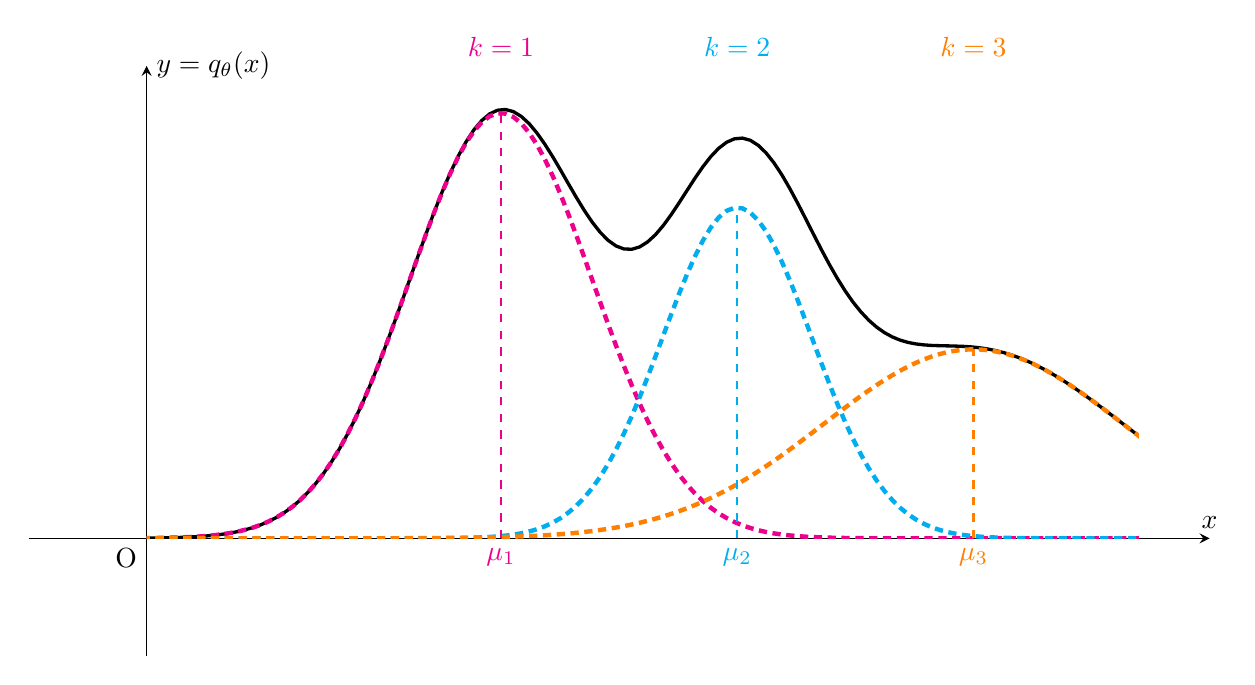
\begin{tikzpicture}[scale=3,samples=300]
    \draw[->,>=stealth,semithick](-0.5,0)--(4.5,0)node[above]{$\vv{x}$};%x軸
    \draw[->,>=stealth,semithick](0,-0.5)--(0,2)node[right]{$y=q_{\theta}(\vv{x})$};%y軸
    \draw(0,0)node[below left]{O};%原点
    \begin{scope} \clip (0,0) rectangle (4.2,2);
      \draw[black,very thick]plot(\x,{4*0.45*exp(-1*pow((\x-1.5),2)/(0.3))+4*0.35*exp(-1*pow((\x-2.5),2)/(0.2))+4*0.2*exp(-1*pow((\x-3.5),2)/(0.8))});
      \draw[densely dashed,magenta,ultra thick]plot(\x,{4*0.45*exp(-1*pow((\x-1.5),2)/(0.3))});
      \draw[densely dashed,cyan,ultra thick]plot(\x,{4*0.35*exp(-1*pow((\x-2.5),2)/(0.2))});
      \draw[densely dashed,orange,ultra thick]plot(\x,{4*0.2*exp(-1*pow((\x-3.5),2)/(0.8))});
    \end{scope}
    \draw[magenta](1.5,2)node[above]{$k=1$};
    \draw[thick,dashed,magenta](1.5,0)node[below]{$\vv{\mu}_1$}--(1.5,4*0.45);
    \draw[cyan](2.5,2)node[above]{$k=2$};
    \draw[thick,dashed,cyan](2.5,0)node[below]{$\vv{\mu}_2$}--(2.5,4*0.35);
    \draw[orange](3.5,2)node[above]{$k=3$};
    \draw[thick,dashed,orange](3.5,0)node[below]{$\vv{\mu}_3$}--(3.5,4*0.20);
  \end{tikzpicture}
  \caption{3つの混合ガウス分布によるモデル$q_{\theta}$(実線)の概念図}
\end{figure}

\subsection{隠れた変数}
混合ガウス分布を考えることで、解析的な計算が可能なままモデルを複雑化することができた。
このような考え方を一般化するために隠れ変数を導入する。
混合ガウス分布は、複数のガウス分布の和によって構成されるモデルであるが、
逆に何らかの$q_{\theta}(\vv{x})$が与えられた際に、それを構成するそれぞれのガウス分布自身を知ることは難しい。
すなわち、モデルを構成するガウス分布は隠れた変数であり、その値を知ることができない。
そのため、データ$\vv{x}$が従うモデル$q_{\theta}(\vv{x})$は、隠れた変数$\vv{z}$によって生成されていると考える:
\begin{equation}
  q_{\theta}(\vv{x}) = \sum_{\vv{z}}q_{\theta}(\vv{x},\vv{z}) = \sum_{\vv{z}}q_{\theta}(\vv{x}|\vv{z})q_{\theta}(\vv{z})\;。
\end{equation}
ここで、$q_{\theta}(\vv{x},\vv{z})$は$\vv{x}$と$\vv{z}$の結合確率であり、$q_{\theta}(\vv{x}|\vv{z})$は$\vv{x}$の$\vv{z}$による条件付き確率である。
先ほどの混合ガウス分布では、$\qty{\vv{\mu}_k,\Sigma_k}$を隠れた変数として生成されるモデルと考えることができる。これを踏まえて、混合ガウス分布を隠れた変数の考え方を用いて再考する。
すなわち、$\vv{\mu}_k,\,\Sigma_k$はデータベクトル$\vv{x}$の成分に依存しないとすると、
\begin{equation}
  q_{\theta}(z) = C_z,\quad q_{\theta}(\vv{x}|z) = \frac{1}{\sqrt{(2\pi)^{N}\det(\Sigma)}}\exp(-\frac{1}{2}(\vv{x}-\vv{\mu}_z)^{\top}\Sigma_{z}^{-1}(\vv{x}-\vv{\mu}_z))
\end{equation}
と表すことができ、混合確率(モデル)は
\begin{equation}
  q_{\theta}(\vv{x},z) = \sum_{z}q_{\theta}(\vv{x}|z)q(z) = \sum_{z}\frac{C_z}{\sqrt{(2\pi)^{N}\det(\Sigma)}}\exp(-\frac{1}{2}(\vv{x}-\vv{\mu}_z)^{\top}\Sigma_{z}^{-1}(\vv{x}-\vv{\mu}_z))
\end{equation}
となる。EMアルゴリズムにおいて、パラメータの偏微分を行って最適化を行った。偏微分による方法を代理関数の下界最大化という立場から考察する。
すなわち、対数尤度関数の代理関数を見つける必要がある。
しかし、混合ガウス分布のモデルのように隠れた変数についての和でモデルが表現されている場合、対数の中に和が出てきて計算することができない。
そのため、
\begin{equation}
  \ln{q_{\theta}(\vv{x})} = \ln\frac{q_{\theta}(\vv{x},z)}{q_{\theta}(z|\vv{x})}
\end{equation}
と変形する。なお、$q_{\theta}(\vv{x},z)=q_{\theta}(z,\vv{x})$を用いた。右辺にある$z$の条件付き確率は未知であるため計算できない。
しかし、適当な分布$r(z)$に従う乱数を用いて期待値を計算してみる:
\begin{equation}
  \sum_{z}r(z)\ln\frac{q_{\theta}(\vv{x},z)}{q_{\theta}(z|\vv{x})} = \sum_{z}r(z)\ln\frac{q_{\theta}(\vv{x},z)}{r(z)}
  -\sum_{z}r(z)\ln\frac{q_{\theta}(z|\vv{x})}{r(z)}\;。
\end{equation}
すると、右辺第二項が変数$z$に関するKL情報量の形になっていることがわかる。したがって、
\begin{equation}
  \ln{q_{\theta}(\vv{x})} = \sum_{z}r(z)\ln\frac{q_{\theta}(\vv{x},z)}{r(z)} + D_{\text{KL}}(r(z)\parallel q_{\theta}(z|\vv{x}))
  \geq \sum_{z}r(z)\ln\frac{q_{\theta}(\vv{x},z)}{r(z)}
\end{equation}
が成立する。すなわち、代理関数として
\begin{equation}
  \sum_{z}r(z)\ln\frac{q_{\theta}(\vv{x},z)}{r(z)}
\end{equation}
を最大化すれば良いことがわかる。代理関数は、期待値計算における確率分布$r(z)$とパラメータ$\theta$に関して最大化することができる。
そのため、まずは
\begin{equation}
  r(z)= q_{\theta}(z|\vv{x})
\end{equation}
として、最大化したい関数と代理関数のギャップを埋める:
\begin{equation}
  \ln{q_{\theta}(\vv{x})} = \sum_{z}q_{\theta}(z|\vv{x})\ln\frac{q_{\theta}(\vv{x},z)}{q_{\theta}(z|\vv{x})}\;。
\end{equation}
右辺は対数の中に和が出てこない形をしているため、パラメータの偏微分が簡単に計算できる。
すなわち、対数尤度関数の最大化は、$r(z)=q_{\theta}(z|\vv{x})$のパラメータ$\theta$を固定した状態で
\begin{equation}
  \max_{\theta}\qty(\frac{1}{n}\sum_{i=1}^{n}\ln{q_{\theta}(\vv{x}_i)})
  = \max_{\theta}\qty(\frac{1}{n}\sum_{i=1}^{n} \sum_{z}q_{\theta}(z|\vv{x}_i)\ln\frac{q_{\theta}(\vv{x}_i,z)}{q_{\theta}(z|\vv{x}_i)})
\end{equation}
を考えることになる。これは$Q$関数
\begin{equation}
  Q(\theta,\theta_0)\coloneqq \frac{1}{n}\sum_{i=1}^{n} \sum_{z}q_{\theta_0}(z|\vv{x}_i)\ln{q_{\theta}(\vv{x}_i,z)}
\end{equation}
を$\theta$について最大化することと等しい。なお、
\begin{equation}
  q_{\theta}(z|\vv{x}_i) = \frac{q_{\theta}(\vv{x}_i,z)}{q_{\theta}(\vv{x}_i)}
  = \frac{q_{\theta}(\vv{x}_i,z)}{\sum_{z}q_{\theta}(\vv{x}_i,z)} = \frac{C_z\exp(\cdots)}{\sum_{z}C_z\exp(\cdots)} = \gamma_{iz}
\end{equation}
となることがわかる。すなわち、$q_{\theta}(z|\vv{x})$を固定したままパラメータ$\theta$を最適化することは、
EMアルゴリズムにおいて負担率$\gamma_{ik}$を固定したままパラメータ$\theta$を最適化したことに対応している。
そのため、$Q$関数の最大化がEMアルゴリズムのパラメータ更新則と同じものを導くことが期待される。実際に、
\begin{equation}
  Q(\theta,\theta_0) = \frac{1}{n}\sum_{i=1}^{n}\sum_{z}\gamma_{iz}\qty[\qty(-\frac{1}{2}(\vv{x}_i - \vv{\mu}_z)^{\top}\Sigma_{z}^{-1}(\vv{x}_i-\vv{\mu}_z)+ \frac{1}{2}\det(\Sigma^{-1}))+\ln{C_z}]
\end{equation}
であることを用いると、
\begin{align}
  \pdv{Q(\theta,\theta_0)}{\vv{\mu}_z}    & = \frac{1}{n}\sum_{i=1}^{n}\gamma_{iz}\qty(\Sigma_z^{-1}(\vv{x}_i-\vv{\mu}_z))=0                                                  &  &
  \Longleftrightarrow \vv{\mu}_z = \frac{\sum_{i=1}^{n}\gamma_{iz}\vv{x}_i}{\sum_{i=1}^{z}\gamma_{iz}}                                                                             \\
  \pdv{Q(\theta,\theta_0)}{\Sigma^{-1}_z} & = \frac{1}{n}\sum_{i=1}^{n}\gamma_{iz}\qty(-\frac{1}{2}(\vv{x}_i-\vv{\mu}_z)(\vv{x}_i-\vv{\mu}_z)^{\top} + \frac{1}{2}\Sigma_z)=0 &  &
  \Longleftrightarrow \Sigma_z = \frac{\sum_{i=1}^{n}\gamma_{iz}(\vv{x}_i-\vv{\mu}_z)(\vv{x}_i-\vv{\mu}_z)^{\top}}{\sum_{i=1}^{z}\gamma_{iz}}
\end{align}
となり、EMアルゴリズムの結果と一致する。また、隠れた変数の最適化も行うことができる。これは、混合ガウス分布における重みづけの係数$q_\theta(z)=C_z$の最適化のことである。
一般に、隠れた変数の束縛条件
\begin{equation}
  \sum_{\vv{z}}q_{\theta}(\vv{z}) = 1
\end{equation}
が成立しているため、拘束付き最適化問題
\begin{equation}
  \max_{C_z}\qty(Q(\theta,\theta_0)+\lambda\qty(\sum_{z}C_z-1)) \eqqcolon \max_{C_z}(Q(\theta,\,\theta_0; C_z))
\end{equation}
を解けば良い。
\begin{equation}
  \pdv{Q(\theta,\theta_0;C_z)}{C_z} = \frac{1}{n}\sum_{i=1}^{n}\frac{\gamma_{iz}}{C_z} + \lambda=0
  \Longleftrightarrow \lambda C_z = -\frac{1}{n}\sum_{i=1}^n \gamma_{iz}
\end{equation}
となる。$z$についての和を取ると、
\begin{equation}
  \lambda = -\frac{1}{n}\sum_{i=1}^n \sum_{z}\gamma_{iz}
\end{equation}
と求まるため、$C_z$について解きなおすと
\begin{equation}
  C_z = \frac{\sum_{i=1}^{n}\gamma_{iz}}{\sum_{i=1}^{n}\sum_{z}\gamma_{iz}}
\end{equation}
と求まる。
このように、隠れた変数の期待値(Expectation)を取る乱数の最適化とパラメータ$\theta$による対数尤度関数の最大化(Maximization)を繰り返すことでモデルの最適化が行える。
これがEMアルゴリズムと呼ばれる理由である。

\section{制限ボルツマンマシン}
計算が可能な範囲でモデルを複雑にするためには、隠れた変数を導入すれば良いということが混合ガウス分布モデルの考察でわかった。
隠れた変数をボルツマンマシンで扱えるようにしたものを制限ボルツマンマシンと呼ぶ。
データ変数を$\vv{x}$、隠れた変数を$\vv{z}$とする。
このとき、ボルツマンマシンにおいてエネルギー関数が
\begin{equation}
  -E_{\theta}(\vv{x},\vv{z})=\vv{x}^{\top}W\vv{z} + \vv{b}^{\top}\vv{x}+\vv{c}^{\top}\vv{z}
\end{equation}
と表されるものを制限ボルツマンマシンと呼ぶ。
これは、データ変数同士の相互作用と隠れた変数同士の相関がなく、データ変数と隠れた変数間の結合だけが存在するようなモデルと考えることができる。
例えば、データと隠れた変数が
\begin{equation}
  \{\vv{x}_1,\,\vv{x}_2,\,\vv{x}_3,\,\vv{x}_4\}:\text{データ}\qquad \{\vv{z}_1,\,\vv{z}_2,\,\vv{z}_3\}:\text{隠れた変数}
\end{equation}
とすると、結合の強さ$W$の制限ボルツマンマシンは以下のようなグラフ構造となる:
\begin{figure}[H]
  \centering
  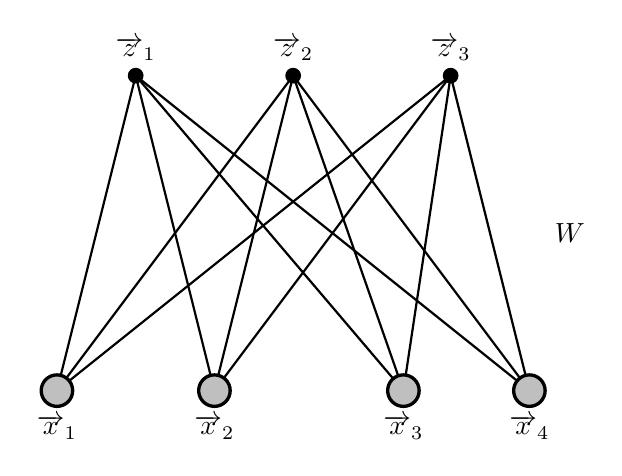
\begin{tikzpicture}[scale=0.4]

    \coordinate(z1)at(-5,10);
    \coordinate(z2)at(0,10);
    \coordinate(z3)at(5,10);
    \coordinate(x1)at(-7.5,0);
    \coordinate(x2)at(-2.5,0);
    \coordinate(x3)at(3.5,0);
    \coordinate(x4)at(7.5,0);

    \foreach\Z in{z1,z2,z3}\foreach\X in{x1,x2,x3,x4}\draw[thick](\Z)--(\X);
    \foreach\Z in{z1,z2,z3}\fill[black](\Z)circle(0.25);
    \foreach\X in{x1,x2,x3,x4}\filldraw[fill=lightgray,very thick](\X)circle(0.50);

    \foreach\i in{1,2,3,4}\draw[black](x\i)node[below=5.5pt]{$\overrightarrow{x}_{\i}$};
    \foreach\j in{1,2,3}\draw[black](z\j)  node[above=2pt]{$\overrightarrow{z}_{\j}$};
    \draw[black](8,5)node[anchor=west]{$W$};
  \end{tikzpicture}
  \caption{制限ボルツマンマシンのグラフ構造}
\end{figure}
\subsection{制限ボルツマンマシンの条件付き独立性}
制限ボルツマンマシンのモデル
\begin{equation}
  q_{\theta}(\vv{x},\vv{z}) = \frac{1}{Z}\exp(\vv{x}^{\top}W\vv{z} + \vv{b}^{\top}\vv{x}+\vv{c}^{\top}\vv{z})
\end{equation}
に対して、データの次元を$N$、隠れた変数の次元を$N_h$とする。
$k=1,\,2,\,\cdots,\,N,\, l=1,\,2,\,\cdots,\,N_h$に対して、
$\vv{u}_k^{\top}$を$W$の$k$行目を取り出した横ベクトル、$\vv{v}_l$を$W$の$l$行目を取り出した縦ベクトルとすると、
\begin{align}
  q_{\theta}(\vv{z}) & = \sum_{\vv{x}=\{1,-1\}^{N}}q_{\theta}(\vv{x},\vv{z}) = \frac{1}{Z}\prod_{k=1}^{N}2\cosh(\vv{u}_k^{\top}\vv{z}+b_k)e^{\vv{c}^{\top}\vv{z}}     \\
  q_{\theta}(\vv{x}) & = \sum_{\vv{z}=\{1,-1\}^{N_h}}q_{\theta}(\vv{x},\vv{z}) = \frac{1}{Z}\prod_{l=1}^{N_h}2\cosh(\vv{v}_l^{\top}\vv{x}+c_l)e^{\vv{b}^{\top}\vv{x}}
\end{align}
が成立する。
したがって、$\vv{x}$の条件付き確率は
\begin{equation}
  q_{\theta}(\vv{x}|\vv{z}) = \frac{q_{\theta}(\vv{x},\vv{z})}{q_{\theta}(\vv{z})}
  = \prod_{k=1}^{N}\frac{\exp(x_k\vv{u}_k^{\top}\vv{z}+b_kx_k)}{2\cosh(\vv{u}_k^{\top}\vv{z}+b_k)} = \prod_{k=1}^{N}q_{\theta}(x_k|\vv{z})
\end{equation}
と計算できる。このように、条件付き確率が各データについての積に分解できるとき、条件付き独立と呼ぶ。
同様にして、$\vv{z}$の条件付き確率は
\begin{equation}
  q_{\theta}(\vv{z}|\vv{x}) = \frac{q_{\theta}(\vv{x},\vv{z})}{q_{\theta}(\vv{x})}
  = \prod_{l=1}^{N_h}\frac{\exp(z_l\vv{v}_l^{\top}\vv{x}+c_lz_l)}{2\cosh(\vv{v}_l^{\top}\vv{x}+c_l)} = \prod_{l=1}^{N_h}q_{\theta}(z_l|\vv{x})
\end{equation}
と計算出来るため、条件付き独立となっている。$q_{\theta}(\vv{z}|\vv{x})$とは、データ$\vv{x}$が与えられたときに隠れた変数$\vv{z}$が従う確率分布であった。
条件付き独立が成立していることから、それぞれの隠れた変数$\vv{z}_{l\in N_h}$を確率分布$q_{\theta}(z_l|\vv{x})$に従ってサンプリングを行うことができる。




\section{マルコフ連鎖モンテカルロ法(MCMC)}

\section{交換モンテカルロ法}

\section{MCMCを用いないボルツマンマシン}

\section{変分オートエンコーダー}

\section{階層変分オートエンコーダ}


\newpage
\section{Appendix}

\subsection{微分に必要な線形代数の公式その1}
$\vv{x}$を$n$次元ベクトル、$A$を$n$次正方行列とする。このとき、$\vv{x}^{\top}A\vv{x}$はスカラーであるため、
\begin{align}
  \dv{\vv{x}}(\vv{x}^{\top}A\vv{x}) & = \dv{\vv{x}}\trace(\vv{x}^{\top}A\vv{x}) = \dv{\vv{x}}\tr(A\vv{x}\vv{x}^{\top})
  = \dv{\vv{x}}\sum_{i,j=1}^{n}A_{ij}(\vv{x}\vv{x}^{\top})_{ji} \notag                                                 \\
                                    & = \sum_{i=1}^{n}\bm{e}_{i}\dv{x_i}\qty(\sum_{k,l=1}^{n}A_{kl}x_lx_k)
  = \sum_{i=1}^{n}\bm{e}_{i}\qty(\sum_{k=1}^{n}A_{ki}x_k + \sum_{l=1}^{n}A_{il}x_l) = (A+A^{\top})\vv{x}
\end{align}
が成立する。なお、$\bm{e}_i$を$i$番目の基底ベクトルとして、$\dv*{\vv{x}} = \sum_{i=1}^{n}\bm{e}_i\dv*{x_i}$であることを用いた。
分散共分散行列は対称行列であるため、
\begin{equation}
  \dv{\vv{x}}(\vv{x}^{\top}\Sigma^{-1}\vv{x}) = 2\Sigma^{-1}\vv{x}
\end{equation}
となる。
\subsection{微分に必要な線形代数の公式その2}
\begin{equation}
  \dv{A_{ij}}(\vv{x}^{\top}A\vv{x})  = \dv{A_{ij}}\tr(A\vv{x}\vv{x}^{\top})
  = \dv{A_{ij}}\sum_{i,j=1}^{n}A_{ij}(\vv{x}\vv{x}^{\top})_{ji} = x_jx_i = (\vv{x}\vv{x}^{\top})^{\top}_{~ij}
\end{equation}
が成立するため、
\begin{equation}
  \dv{A}(\vv{x}^{\top}A\vv{x})  = \vv{x}\vv{x}^{\top}
\end{equation}
となる。
\subsection{微分に必要な線形代数の公式その3}
determinantの余因子展開
\begin{equation}
  \det(A) = \sum_{j=1}^{n}(-1)^{i+j}A_{ij}m_{ij}\quad(m_{ij}\text{は$A\text{の}(i,j)$小行列式})
\end{equation}
を用いると、
\begin{equation}
  \qty(\dv{A}\det(A))_{ij} = \dv{A_{ij}}\sum_{j=1}^{n}(-1)^{i+j}A_{ij}m_{ij}=(-1)^{i+j}m_{ij}
\end{equation}
となる。さらに、余因子行列$\tilde{A}$を用いて$\det(A) = A\tilde{A}$と表されるため、
\begin{equation}
  \dv{A}\ln{\det(A)} = \frac{1}{\det(A)}\dv{A}\det(A) = \frac{1}{\det(A)}\tilde{A}^{\top} = (A^{-1})^{\top}
\end{equation}
を得る。したがって、
\begin{equation}
  \dv{\Sigma^{-1}}\ln{\det(\Sigma)} = -\Sigma^{\top} = -\Sigma
\end{equation}
となる。

\end{document}